\chapter{Desarrollo de la Aplicación}
\label{desarrollo-capitulo}
%En el presente capítulo se presenta, de forma detallada, cómo fue el desarrollo del proyecto y finaliza con una revisión de dificultades técnicas y los resultados del proyecto.

El presente capítulo describe las etapas del desarrollo de la aplicación. Además se presentan las dificultades técnicas encontradas a lo largo del mismo y el resultado final alcanzado.

El desarrollo se dividió en tres fases:

\begin{enumerate}
    \item Fase de Inicio.    
    \item Fase de Implementación.
    \item Fase de Cierre.
\end{enumerate}

Previo a la realización de estas fases, se llevó a cabo una fase para la descarga e incialización de las herramientas a ser utilizadas en el desarrollo de la aplicación. Además se crearon las cuentas para el manejo de  los repositorios del proyecto

Cada fase posee sus propios objetivos generales y específicos, la fase de implementación contempla también los \textit{Sprint} realizados siguiendo la metodología seleccionada.

\section{Fase de Inicio}
    
    \textbf{\underline{Objetivo General:}}
    Llevar a cabo el levantamiento de requerimientos e identificación de los módulos a desarrollar en el proyecto.
    
    \textbf{\underline{Objetivos Específicos:}}
    \begin{itemize}
        \item Levantamiento de los requerimientos del sistema.
        \item Identificación de los módulos que conformarán el sistema a desarrollar.
        %\item Descarga y configuración de Eclipse, JSON, Hibernate, Liquibase, Maven, AngularJS, Apache y Tomcat.
        %\item Creación de cuentas para el manejo de los repositorios del proyecto y \textit{Product Backlog}.
        \item Creación del \textit{Product Backlog}.
        \item Elaboración del diagrama inicial de base de datos. %y casos de uso.
        \item Evaluación de restricciones y riesgos por parte del equipo de desarrollo.
    \end{itemize}
    
    En esta fase se realizó, en conjunto con el ing. Juán Albarrán, el levantamiento de los requerimientos funcionales y no funcionales del sistema, dichos requerimientos fueron:
    
    \subsection{Requerimientos Generales}
    \begin{itemize}
        \item El sistema debe poseer mecanismos de autenticación para la verificación de identidad.
        
        \item El sistema debe proveer una plataforma de almacenamiento de historiales médicos con asociaciones entre la empresa en la que trabaja el paciente, la sucursal o ``centro de costos"\footnote{Se usa el término \textit{Centro de Costos} para referirse a una sucursal o sede donde haya personal tabajando.} en el cual trabaja el paciente al momento de la consulta.
        
        \item Mantener los historiales a través del tiempo, sin importar los cambios de ``centro de costos", que presente el paciente, ni el médico que lo atienda.
        
        \item En casos de algún cambio en el centro de costos donde trabaja el paciente, se deberán especificar como terminación o renovación de contratos de parte de los usuarios y la empresa.

    \end{itemize}        
        
        Todo esto con la finalidad de poder realizar cruces de información e investigación de causas de enfermedades tomando en cuenta los lugares de trabajo y las tareas desempeñadas por los trabajadores.
        
    \subsection{Requerimientos Específicos}
    
    \begin{itemize}
        \item \textbf{\underline{Usuarios:}}
        
        Fue modelado como ``Usuario" todo aquel empleado de una empresa registrada en el sistema. Para efectos del presente proyecto, los usuarios son los trabajadores de las empresas. Se hace una diferencia especial a dos tipos específicos de usuario: el doctor y el paciente (no excluyentes) que son la línea principal de trabajo del sistema. El sistema debe ser capaz de mantener una base de datos de usuarios con los atributos especificados en el Apédice \ref{ere}.
        
        La categoría de ``Doctor" en una empresa se refiere al personal médico calificado para realizar consultas y diagnósticos médicos, por consecuencia será representado como un contrato especial y, sin discriminación por la especialidad o nivel de instrucción del mismo, será almacenado en el sistema con el nombre de ``Doctor". En la sección de almacenamiento de los datos del doctor, será  almacenada la información específica del mismo.
        
        Los ``Pacientes" por otro lado representan a todo el personal que haya sido atendido y tenga su historia médica registrada en el sistema. Cabe destacar que un ``Doctor" puede también ser paciente, aunque no puede ser su propio paciente.
        
        \item \textbf{\underline{Historial Médico:}}
        
        El historial médico de un paciente se realiza al momento de la primera consulta que sea registrada en el sistema, en ese momento de registran:
        
        \begin{enumerate}
            \item Antecedentes o Trasfondos: Enfermedades diagnosticadas previamente al paciente así como predisposiciones a enfermedades hereditarias.
            \item Hábitos: Son actividades regulares del paciente. Pueden variar en tipo y frecuencia. Éstos pueden ser habitos recomendados o perniciosos para el paciente. La finalidad es que las investigaciones de enfermedades ocupacionales puedan descartar los hábitos de los pacientes como factores.
            \item Alergias: También se registran alergias diagnosticadas al paciente. Se realiza en una sección a parte de los trasfondos debido a que las alergias poseen características específicas y se manifiestan sólo con la presencia del alérgeno\footnote{Según el diccionario de la RAE: \textit{alérgeno, na}: 1. adj. Perteneciente o relativo a los alérgenos. 2. m. Sustancia antigénica que induce una reacción alérgica en un organismo.} correspondiente.
            \item Vacunas: Por último ser registran las vacunas que posee el paciente detallando el nombre y la potencia en caso en que aplique (vacunas de varias dosis o refuerzos).
        \end{enumerate}
        
        El usuario debe estar previamente registrado y contratado por la empresa que contrata al doctor para poder crearse su historial médico.
        
        \item \textbf{\underline{Consultas Médicas:}}
        \label{consultas-datos}
        
        Una vez creado el historial médico pueden realizarse consultas médicas. En ellas se registrará la información recogida durante dicha consulta y se almacenará en el sistema.
        
        Basándose en la información recopilada por Globinsoft S.A. para su proyecto ``HxPlus" (principal antecedente del presente proyecto), queda establecida la estructura de una consulta de la siguiente forma:
        
        \begin{enumerate}
            \item \textit{SoapNote} (nota de revisión): Usada por los médicos para organizar las consultas y que consta de:
            \begin{enumerate}
                \item Subjective: Información subjetiva, comunmente redactada en lenguaje informal, que contiene lo que el paciente describe, dolencias y síntomas presentados.
                \item Objective: Información objetiva recopilada por el médico durante la consulta. Redactada en lenguaje formal.
                \item Assessment: Comentarios u observaciones realizados por el médico.
                \item Plan: Plan acción a realizar para tratar las dolencias.
            \end{enumerate}
            \item Diagnóstico(s): Uno o varios diagnósticos realizados por el médico en la consulta.
            \item Instrucción(es): Una o varias instrucciones. Acciones que deben ser llevadas al pie de la letra en cuanto a conductas o hábitos del paciente, se incluye en este apartado regulaciones alimenticias y recomendaciones periódicas.
            \item Prescripción(es): Instrucciones de uso de medicamentos registrados en el sistema junto con la información de dicho medicamento. Con esto se podrán generar los récipes médicos para la adquisición de fármacos que así lo requieran.
            \item Signos Vitales: Se registran los signos vitales recabados en la consulta. Dado que puede variar los signos vitales pertinentes entre las distintas especialidades de la medicina, se deja a juicio del médico tratante qué signos vitales serán tomados en la consulta.
            \item Solicitud y Recepción de exámenes médicos: En la primera se registra una solicitud de un examen dado. En una futura consulta puede darse por recibido en el sistema el examen médico y adjuntar el archivo respectivo para su almacenamiento. Se puede solicitar o recibir más de un examen médico por consulta.
        \end{enumerate}
        
        El sistema debe ser capaz de almacenar y desplegar esta información ordenada cronológicamente a partir de la consulta médica más reciente.
        
        \item \textbf{\underline{Reportes Médicos:}}
        
        El sistema debe poder generar de manera automática los reportes médicos con la información recopilada en las consultas a solicitud del médico.
    \end{itemize}
    
    Todos estos requerimientos fueron archivados en notas para la realización del \textit{Product Backlog} utilizando el sistema Trello y se enlazó con la pizarra creada por el \textit{Scrum Manager} para la gestión del proyecto.
    
    Se dividió el proyecto en ``módulos" y éstos a su vez en ``vistas" las cuales pasaron a ser la unidad granular deseada para el manejo del proyecto, quedando así la primera versión de la lista del producto de la siguiente forma:
    
    \begin{enumerate}
        \item \textbf{\underline{Módulo de Autenticación:}}
        
        \begin{itemize}
            \item Vista de autenticación: Incluye inicio y cierre de sesión dentro del sistema.
        \end{itemize}
        
        \item \textbf{\underline{Módulo de Gestión de Usuarios:}}
        
        \begin{itemize}
            %\item Vista de Agregar Usuario: Formulario de creación de usuarios nuevos en el sistema.
            \item Vista de Lista de Usuarios: Lista de los usuarios registrados en el sistema. Esta vista será refinada en el futuro para que haga discriminación entre usuarios por empresa (ej. un usuario de una empresa A no podrá ver la lista de otra empresa B ni éstos aparecerán en su lista).
            \item Vista de Detalles de Usuario: Vista de los datos personales de un usuario.
            \item Vista de Edición de Usuario: Formulario lleno con los datos personales de un usuario.
        \end{itemize}
        
%        \item \textbf{\underline{Módulo de Doctores:}}
%        \begin{itemize}
%            \item Vista de Agregar Doctor: Formulario para el registro de un nuevo dorctor en la empresa.
%            \item Vista de Lista de Doctores: Lista con los doctores contratados por una empresa.
%            \item Vista de Detalles de Doctor: Vista de los datos característicos de un doctor.
%            \item Vista de Edición de Doctor: Formulario lleno con los datos profesionales de un doctor dado. Se usa para la actualización de dichos datos.
%        \end{itemize}
        
        \item \textbf{\underline{Módulo de Pacientes:}}
        \begin{itemize}
            \item Vista de Añadir Nuevo Paciente: Al añadir un nuevo paciente, el doctor puede añadir un nuevo paciente a su lista de pacientes atendidos y el mismo puede provenir de las listas de usuarios atendidos previamente y que estén contratados por la empresa o ser un paciente totalmente nuevo, en tal caso pasaría a la siguiente vista.
            \item Vista de Lista de Pacientes Atendidos: El doctor tiene a su disposición una lista de pacientes que ha atendido con anterioridad, ordenada por fecha de última consulta médica y se mostrarán los pacientes atendidos más recientemente primero.
            \item Vista de Creación de Historia Médica: Formulario con el cual se añaden los datos necesarios para la creación de una nueva historia médica al sistema. Usado en el caso de que un paciente esté siendo atendido por primera vez desde su registro en el sistema (no importa si ha cambiado de puesto de trabajo, sólo se discrimina por el puesto actual).
        \end{itemize}
        
        \item \textbf{\underline{Módulo de Consultas Médicas:}}
        \begin{itemize}
            \item Vista de Historial de Consultas Médicas del Paciente: Una lista de las consultas que ha tenido el paciente ordenadas cronológicamente empezando desde la última consulta.
            \item Vista de Agregar Consulta Médica: Formulario con los datos requeridos para almacenar una consulta médica nueva.
            \item Vista de Revisión de Consulta Médica: En esta vista se despliegan los datos almacenados de una consulta médica ya realizada. También se accede a los archivos previamente almacenados (exámenes médicos recibidos) y a la funcionalidad de generación de reportes.
            \item Vista de Generación de Reportes Médicos: En esta vista de podrán elegir los reportes que serán generados por el sistema.            
        \end{itemize}
    \end{enumerate}
    
    Todo esto quedó plasmado en el sistema de pizarras de Trello asociado a la cuenta del equipo de desarrollo.
    
    Basándose en los requerimientos recopilados, el equipo de desarrollo, realizó un diagrama de base de datos el cual a su vez fue modificado durante el desarrollo del proyecto. La versión final del mismo puede ser consultado en el Apéndice \ref{ere}.
    
    Del análisis de riesgos del proyecto, se obtuvo la siguiente lista de riesgos:
    
    \begin{enumerate}
        \item \textbf{Equipo de desarrollo pequeño:} Dado que se cuenta con un sólo integrante del equipo de desarrollo los avances en la implementación del proyecto deben ser pequeños con la intención de que sean funcionales y estén probados.
        \item \textbf{Falta de diversidad en el conocimiento:} También por ser un grupo pequeño, pueden surgir, durante el desarrollo, impedimentos por falta de dominio de las herramientas. En tal caso se deberá realizar una fase de capacitación para las fases impedidas lo cual podría retrasar las entregas.
        \item \textbf{Tiempo dedicado a los \textit{Sprint}:} Si los \textit{Sprint} son establecidos en una o dos semanas, los avances podrán verse rápidamente, aunque serían poco avance. Por otro lado, mantener el tiempo de \textit{Sprint} en tres o cuatro semanas, se verían pocos avances y la retroalimentación sería escasa. Para solventar tal riesgo, se designó un tiempo de \textit{Sprint} variable, quedando establecido un tiempo de dos semanas para aquellas vistas en las que el equipo de desarrollo no precise capacitación y de tres a cuatro semanas para las que si sea necesaria la capacitación.
    \end{enumerate}
    
    En paralelo a la realización de este trabajo, se realizó la descarga Eclipse Kepler, descargado desde la página oficial de Eclipse\cite{ECLIPSE-eclipseorg}, Apache, Tomcat (ambos descargados de \cites{APACHE-maven}{APACHE-tomcat} respectivamente) y las librerías de AngularJS.
    
    Se procedió a la configuración de Maven y se agregaron las dependencias iniciales para usar \textit{SPRING} como \textit{framework}, Hibernate y Liquibase como gestores de comunicación con la base de datos y configurar la base de datos con las credenciales de MySQL asignadas para el desarrollo del proyecto.
    
    \begin{table}[h!]
        
        \begin{center}
            \begin{tabular}{|l|l|l|}\hline
                Grupo & Artefacto & Versión \\\hline
                org.springframework & spring-core & 4.1.2.RELEASE \\\hline
                org.springframework & spring-orm & 4.1.2.RELEASE \\\hline
                org.springframework & spring-webmvc & 4.1.2.RELEASE \\\hline
                mysql & mysql-connector-java & 5.1.9 \\\hline
                org.liquibase & liquibase-plugin & 1.6.1.0 \\\hline
            \end{tabular}
        \end{center}
        
        \caption{Artefactos de Maven: Spring}
        \label{artefactos-spring}
    \end{table}
    
    Aunque, en lo referente a liquibase, se utilizó un plugin, no una librería. Ver cuadro \ref{artefactos-spring}.
    
    Se realizaron los cambios dentro del archivo ``occupational-servlet.xml" que permiten el uso de anotaciones para el direccionamiento interno de los procesos.
    
    Usando los repositorios de Maven se descargaron las librerías necesarias de JSON para la comunicación. Las dependencias descargadas fueron del grupo \textit{com.fasterxml.jackson.core}, las enumeradas en el cuadro \ref{artefactos-json}.
     
    \begin{table}[h!]
         
        \begin{center}
            \begin{tabular}{|l|l|}\hline
                Artefacto & Versión \\\hline
                jackson-core & 2.2.2 \\\hline
                jackson-annotations & 2.2.2 \\\hline
                jackson-databind & 2.2.2 \\\hline                   
            \end{tabular}
        \end{center}
        
        \caption{Artefactos de Maven: JSON}
        \label{artefactos-json}
    \end{table}
    
    También, usando Maven, fueron descargadas las librerías de Hibernate que usan JPA como API para comunicarse con la base de datos (cuadro \ref{artefactos-hibernate}).
    
    \begin{table}[h!]
        
        \begin{center}
            \begin{tabular}{|l|l|l|}\hline
                Grupo & Artefacto & Versión \\\hline
                org.hibernate.javax.persistence & hibernate-jpa-2.0-api & 1.0.1.Final \\\hline
                org.hibernate.common & hibernate-commons-annotations & 4.0.4.Final \\\hline
                javax.persistence & persistence-api & 1.0.2 \\\hline
                org.hibernate & hibernate-entitymanager & 4.1.9.Final \\\hline
                org.springframework.data & spring-data-jpa & 1.8.1.RELEASE \\\hline
            \end{tabular}
        \end{center}
        
        \caption{Artefactos de Maven: Hibernate}
        \label{artefactos-hibernate}
    \end{table}
    
\section{Fase de Implementación} 

En esta fase se realizó en sí el desarrollo del sistema. Hubo modificaciones en el diagrama de base de datos (versión final en Apédice \ref{ere-diagrama}) y, los requerimientos que cambiaron, se reflejaron en el \textit{product backlog} conforme fueron sucediendo.

La implementación se subdividió en Sprints y, como se menciona anteriormente, estos fueron de duración variable.

Cabe destacar que dado que los módulos referentes al manejo de empresas (``Compañía", ``Agregar Usuario", ``Contratos" y la gestión de doctores) están por fuera del alcance del proyecto, se utilizó una base de datos de pruebas generada exclusivamente para tal fin. También fueron generados datos de prueba para medicamentos y laboratorios, por las mismas razones expresadas con anterioridad.

    \subsection{Primer Sprint: Vista de Autenticación de Usuarios}
    Se implementó la funcionalidad de autenticación siguiedo los parámetros de autenticación basada en \textit{tokens}, para ello se agregó al ``pom.xml"\footnote{Ver punto \ref{tecno-maven}} las dependencias requeridas para la autenticación. Ver cuadro \ref{artefactos-tba}
    La clave usada por el servidor fue una clave generada en tiempo de ejecución para que la misma fuera cambiante y mejorar la seguridad. Sin embargo, la clave, una vez generada se mantiene igual mientras el servidor esté en funcionamiento. Ver figura \ref{Autenticación}.
    
    \begin{figure}[htbp!]
        \begin{center}
            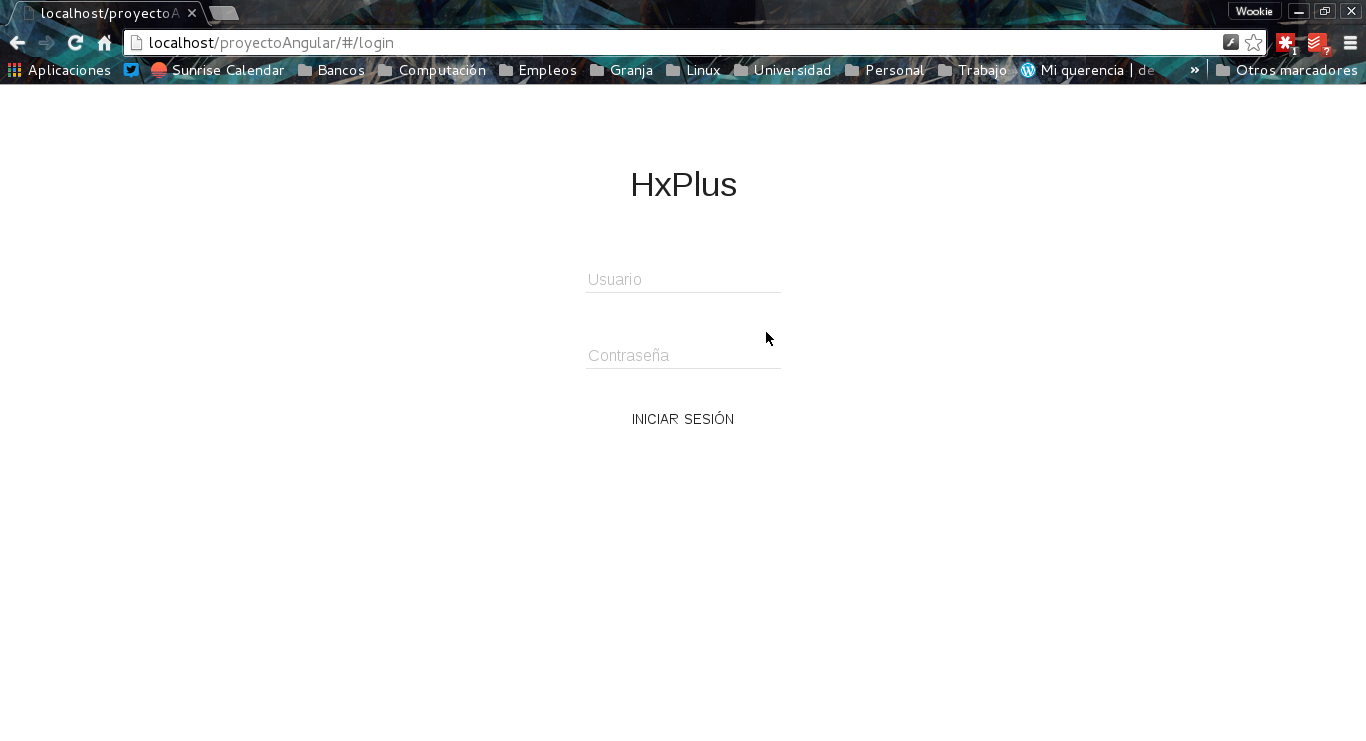
\includegraphics[width=.9\textwidth]{figures/p1}
        \end{center}
        \caption{Pantalla de Autenticación de usuarios}
        \label{Autenticación}
    \end{figure}
    
    \begin{table}[h!]
        
        \begin{center}
            \begin{tabular}{|l|l|l|}\hline
                Grupo & Artefacto & Versión \\\hline
                io.jsonwebtoken & jjwt & 0.5.1 \\\hline
            \end{tabular}
        \end{center}
        
        \caption{Artefactos de Maven: Autenticación}
        \label{artefactos-tba}
    \end{table}
    
    Las pruebas sobre esta vista fueron realizadas evaluando la generación del \textit{token} de parte del servidor en \textit{back end} y su posterior uso para el acceso a las demás páginas del sistema. La ficha fue generada con éxito y verificado el cambio de ficha en cada inicio de sesión, se dió la aprobación de la vista para proseguir al siguiente Sprint.
    
%    \subsection{Segundo Sprint: Vista de Agregar Usuario}
%    
%    En esta vista se buscó crear un formulario con los datos de un usuario nuevo que serán agregados al sistema. Los datos para el mismo fueron:
    
%    \begin{itemize}
%        \item Nombre de usuario: El apodo que tendrá el usuario en el sistema.
%        \item Contraseña: La contraseña que será utilizada para verificar la identidad del usuario. Se reqiuere que sea introducida dos veces al sistema para evitar errores posteriores.
%        \item Cédula de Identidad: El número de cédula es el documento de identificación del usuario en el país.
%        \item RIF: Registro de información fiscal. También es un método de identificación del usuario en el país.
%        \item Nombre: Indica el primer nombre del usuario. No se hace mención al segundo nombre dado que no es estrictamente necesario para el sistema y sería una carga extra para la transferencia de datos.
%        \item Apellido: Indica el primer apellido del usuario.
%        \item Sexo.
%        \item Fecha de nacimiento.
%        \item Correo Electrónico: Correo electrónico del usuario al cual contactarle en caso de ser necesario. También es usado para verificar la identidad del usuario y evitar que sea registrado dos veces en el sistema.
%        \item Dirrección: La dirección de habitación del usuario.
%        \item Número de Teléfono: El número de teléfono al que se pueda contactar al usuario.
%    \end{itemize}
    
%    A este Sprint se le asignó un tiempo de dos semanas debido a que, a pesar se la sencillez del mismo, el equipo de desarrollo no poseía los conocimientos técnicos específicos para el manejo de AngularJS y requirió capacitación previa para solventarse. Para ello se utilizó como referencia \cite{CODESCHOOL-main} en su curso ``Shaping up with Angular.js" que hace referencia al manejo de AngularJS desde el diseño de UI hasta manejo de los datos del lado del cliente.
    
%    Las pruebas fueron realizadas usando los siguientes criterios:
    
%    \begin{enumerate}
%        \item Agregar un usuario con un apodo ya existente.
%        \item Agregar un usuario con un número de cédula o RIF ya existentes.
%        \item Agregar un usuario sin alguno de los campos requeridos (nombre de usuario, contraseña, primer nombre, primer apellido, número de cédula y correo electrónico).
%    \end{enumerate}
    
    \subsection{Segundo Sprint: Vista de Lista de Usuarios}
    
    Esta vista contiene una lista con los nombres de los usuarios registrados en el sistema. Para el alcance del sistema se implementó una lista general sin discriminaciones sobre dicha lista y fue utilizada en las pruebas de la vista de ``Detalles de Usuario". Se plantea que a futuro sea utilizada por usuarios especiales dentro del sistema y que manejen dichas listas dentro de una empresa.
    
    A este Sprint se le asignó una semana de lapso para su entrega dada la importancia relativamente baja de la vista no se refinó y su UI está muy poco refinada.
    
    Las pruebas de la vista se basaron en el orden de aparición de los usuarios (ordenados alfabeticamente) y la actualización de la lista al agregar un nuevo usuario.
    
    \subsection{Tercer Sprint: Vista de Detalles de Usuario}
    
    Esta vista es la muestra de los datos ingresados al sistema del usuario elegido.
    
    A este Sprint, debido a su simpleza, se le dedicó sólo una semana de tiempo para realizar las pruebas necesarias.
    
    Por ser una vista sencilla, las pruebas se realizaron correlacionando los datos de los usuarios con lo que se muestra en pantalla y la aceptación de UI por parte del \textit{product owner}.
    
    \begin{figure}[htbp!]
        \begin{center}
            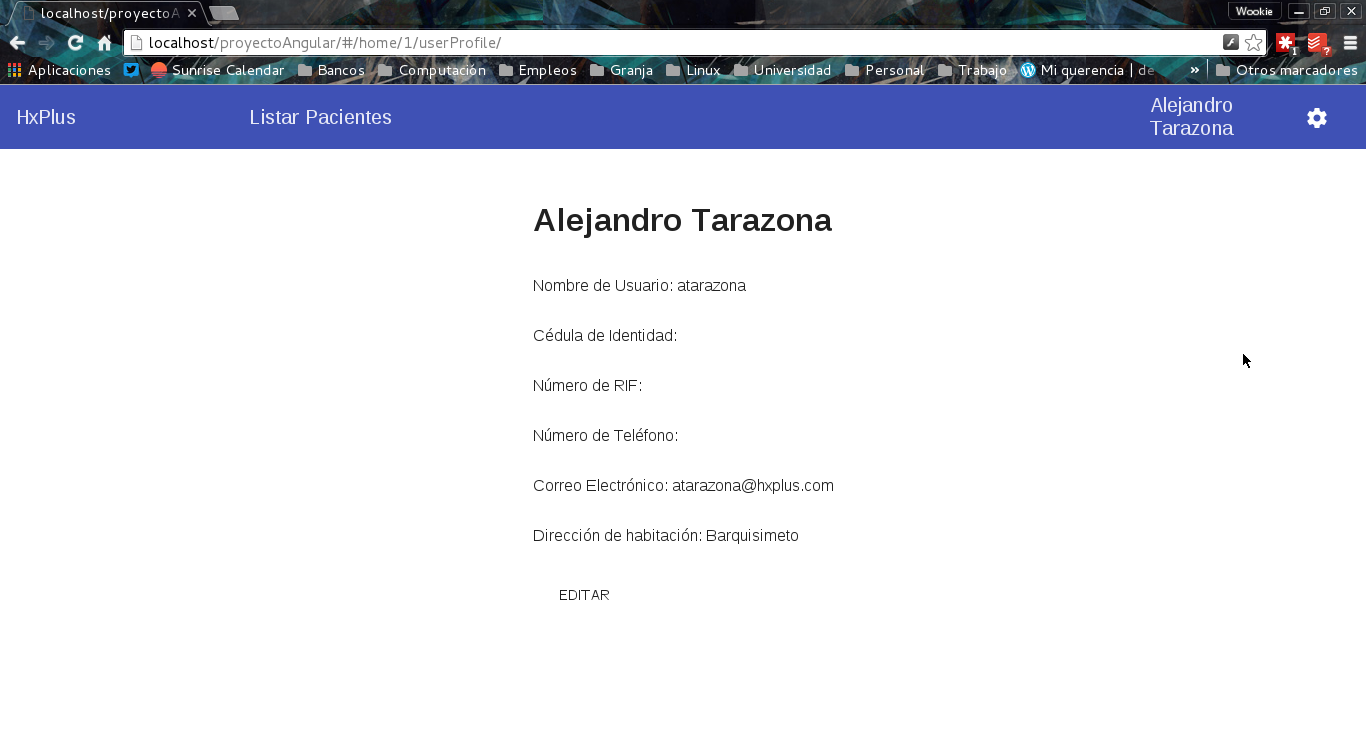
\includegraphics[width=.9\textwidth]{figures/p3}
        \end{center}
        \caption{Pantalla de Revisión de Usuario.}
        \label{Revisión}
    \end{figure}
    
    \subsection{Cuarto Sprint: Vista de Edición de Usuario}
    
    Esta vista muestra un formulario, similar al formulario de registro de usuario, lleno previamente con los datos  previamente registrados. Si el formulario cambia y estos cambios son enviados, el sistema los almacena y regresa a la vista anterior, en caso de éxito, y muestra los datos actualizados del usuario. En caso de algún fallo, el sistema debe dar el mensaje correspondiente al cambio ilegal y mantenerse en la vista con los datos originales del usuario. En caso de modificaciones de la contraseña, el usuario no podrá ver la contraseña previa y el campo estará vacío; este campo se llenará en caso de desear modificarla y se necesita también una verificación de doble escritura de la contraseña para tal fin.
    
    Las pruebas de esta vista fueron:
    \begin{enumerate}
        \item\label{required} Alterar la información del usuario eliminando campos requeridos (nombre de usuario, contraseña, primer nombre, primer apellido, número de cédula y correo electrónico).
%        \item\label{password} Cambiar la contraseña con errores en la doble verificación de escritura.
        \item\label{repeated} Cambiar el nombre de usuario, número de cédula o correo electrónico por valores ya registrados en el sistema.
        \item\label{no-alter} No alterar ningún dato del usuario y enviar el formulario con los datos previos usando el botón de envío de datos.
        \item\label{details} Verificar que los datos fuesen actualizados en la vista anterior en caso de haber verificaciones válidas en el usuario dado.
    \end{enumerate}
    
    A partir del caso \ref{repeated} se detectó que el sistema realizaba una modificación completa del usuario en la base de datos con los datos enviados en el formulario, lo cual podría devenir en problemas de procesamiento a futuro con grandes cargas de datos y es innecesario en el caso \ref{no-alter} por la misma naturaleza de la no modificación. Se acordó, en el siguiente Sprint, revisar esta funcionalidad.
    
    \begin{figure}[htbp!]
        \begin{center}
            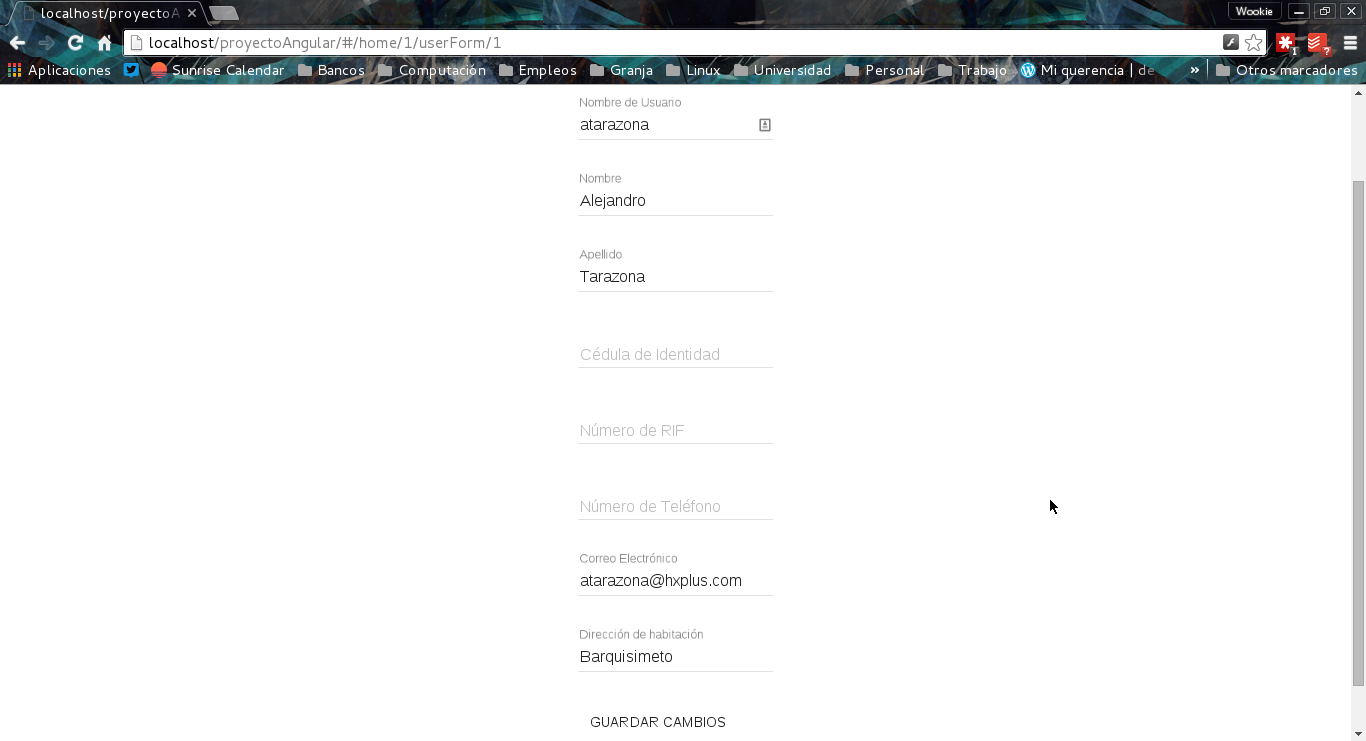
\includegraphics[width=.9\textwidth]{figures/p5}
        \end{center}
        \caption{Pantalla de Edición de Usuario.}
        \label{Edición}
    \end{figure}
    
    A este Sprint, dada la poca complejidad que presenta, se le asignó una semana de duración pero, debido a los errores encontrados en la implementación, se le asignó una semana adicional de revisión adicional dentro del siguiente Sprint.
    
%    \subsection{Quinto Sprint: Vista de Agregar Doctor}%
%    \subsection{Sexto Sprint: Vista de Lista de Doctores}
%    \subsection{Sexto Sprint: Vista de Detalles del Doctor}
%    \subsection{Septimo Sprint: Vista de Edición de Doctor}
    \subsection{Quinto Sprint: Vista de Añadir Nuevo Paciente y Revisón de la Edición de Usuario}
    
    Se realizó la revisión de la ``Vista de Edición de Usuario" debido a que presentaba sobrecarga de datos y en el caso de la no modificación del usuario se reescribían los datos con los mismos valores. El problema fue solventado agregando un detector de cambios con el cual sólo los datos modificados son enviados en el formulario, con esto se logra, no sólo reducir la cantidad de datos enviados al servidor si no que también se elimina la sobrecarga en caso de enviar un formulario con datos idénticos a los que fueron recibidos.
    
    Por otro lado, en la ``Vista de Añadir Nuevo Paciente", el doctor tiene la opción de elegir entre:
    
    \begin{enumerate}
        \item\label{list} Un paciente que ya posea historia médica en el sistema:\\
        Se creó una lista de pacientes cuyos historiales médicos estén registrados en el sistema y serán agregados a la lista de pacientes del doctor.
        \item\label{new} Crear la historia médica de un usuario, ya registrado, que no la posea.\\
        Para este caso se planificó agregar un botón de redirección a la ``Vista de Crear Historia Médica", descrita posteriormente, y que actualizaría la lista de pacientes con historia médica y dejaría en selección el nuevo paciente ya creado.
    \end{enumerate}
    
     Para este Sprint la fase de pruebas de esta vista fue aceptación de la UI y revisión de la acción mencionada en el punto \ref{list} dentro de la base de datos dado que no se cuenta con la vista necesaria y esta será desarrollada en el próximo Sprint.
    
    Se dedicó, en total, dos semanas a este Sprint, dejando para futuros Sprint las pruebas mencionadas.
    
    \begin{figure}[htbp!]
        \begin{center}
            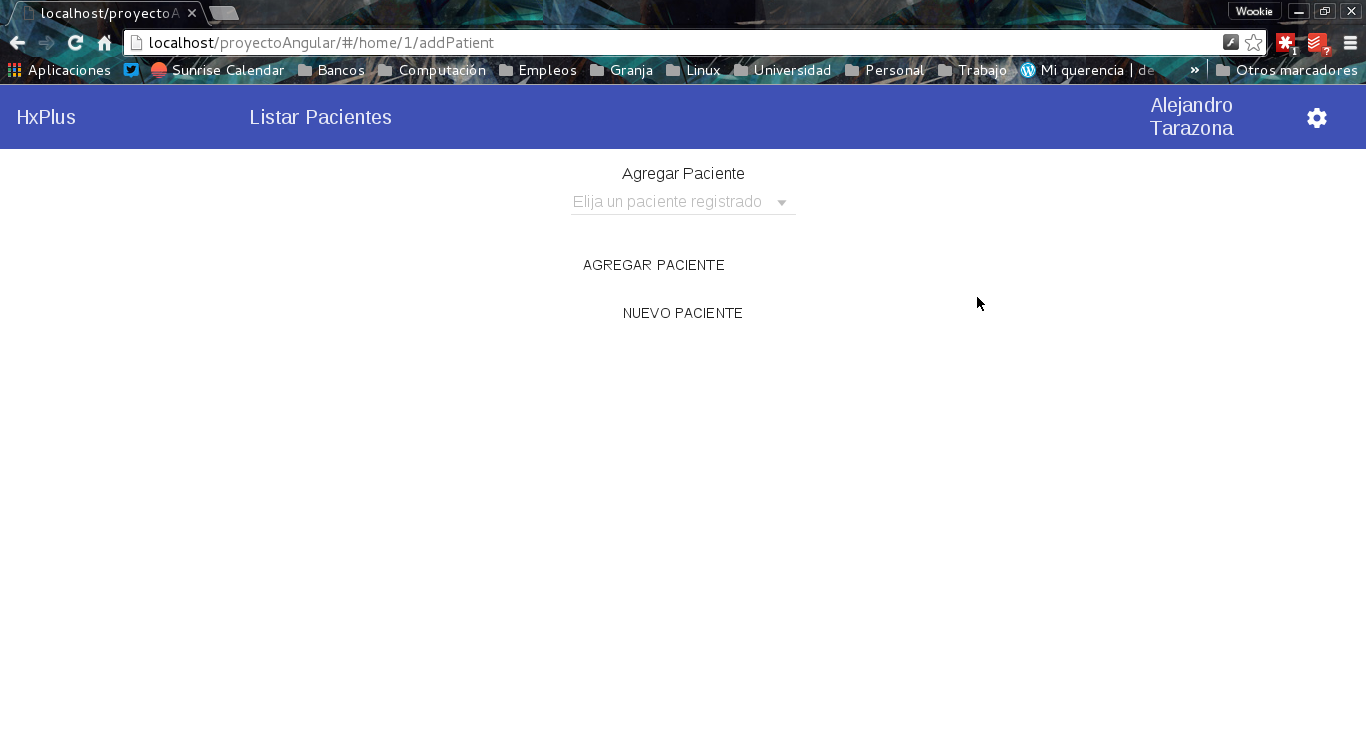
\includegraphics[width=.8\textwidth]{figures/p8}
        \end{center}
        \caption{Vista de Agregar pacientes que ya han sido atendidos por algún médico.}
        \label{Agregar}
    \end{figure}
    
    \subsection{Sexto Sprint: Vista de Lista de Pacientes Atendidos}
    
    En esta vista se presentan por orden alfabético los pacientes que han sido atendidos por el doctor. Además, se presenta la opción de revisar su historial médico con lo cual se desplegará la ``Vista de Historial de Consultas Médicas del Paciente" (ver punto \ref{historial-medico}).
    
    Esta vista se usó como referencia para las pruebas de la ``Vista de Agregar Nuevo Paciente" para revisar que la agregación estaba siendo realizada exitosamente.
    
    Para este Sprint se dedicó una semana y las pruebas se basaron en la respuesta de la vista ante los cambios realizados por la vista mencionada y en la aceptación de la UI.
    
    \begin{figure}[htbp!]
        \begin{center}
            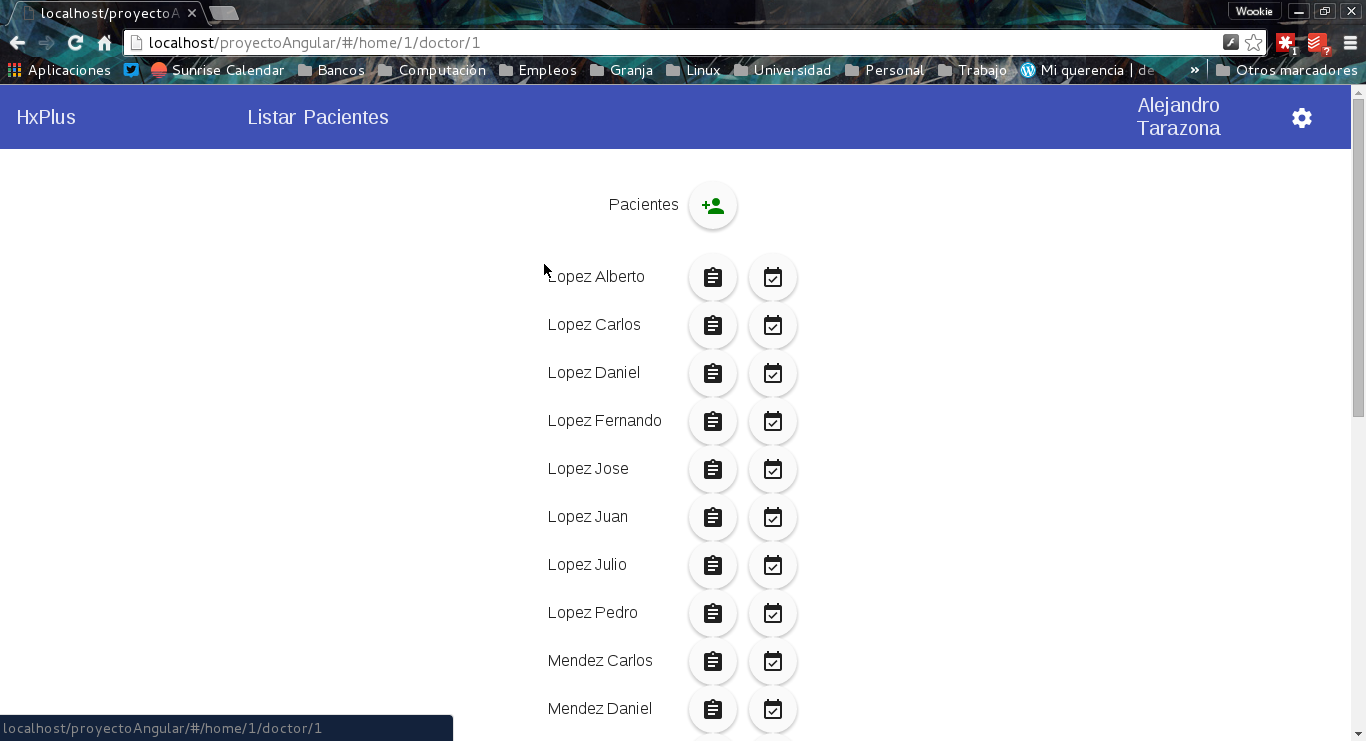
\includegraphics[width=.9\textwidth]{figures/p6}
        \end{center}
        \caption{\label{Pacientes}Lista de Pacientes del Médico}
    \end{figure}
    
    \subsection{Septimo Sprint: Vista de Creación de Historia Médica}
    
    En esta vista se presenta un formulario dinámico\footnote{Flexible en la cantidad de valores que puede aceptar un mismo campo. Puede verse como un ejemplo de un campo multivaluado de un diagrama ER-E} con los campos requeridos para la creación de la historia médica del paciente.
    
    Los campos que admiten más de un sólo valor son:
    \begin{itemize}
        \item Alergias.
            \begin{itemize}
                \item Nombre
                \item Descripción
                \item Severidad
            \end{itemize}
        \item Hábitos.
            \begin{itemize}
                \item Nombre
                \item Frecuencia
            \end{itemize}
        \item Vacunas.
            \begin{itemize}
                \item Nombre
                \item Potencia
            \end{itemize}
    \end{itemize}
    
    Se realizó la subdivisión de acuerdo a los avances realizados por Globinsoft S.A. y están encapsuladas de tal forma que se pueden agregar o eliminar de forma independiente una alergia, un hábito o una vacuna a la lista respectiva sin la necesidad de refrescar o recargar la página. Todos los datos recaudados son enviados una y sólo una vez al servidor una vez seleccionada la opción de envío del formulario.
    
    Las enfermedades diagnosticadas previamente son un único valor dado que puede no ser precisa la información suministrada por el paciente.
    
    \begin{figure}[htbp!]
        \begin{center}
            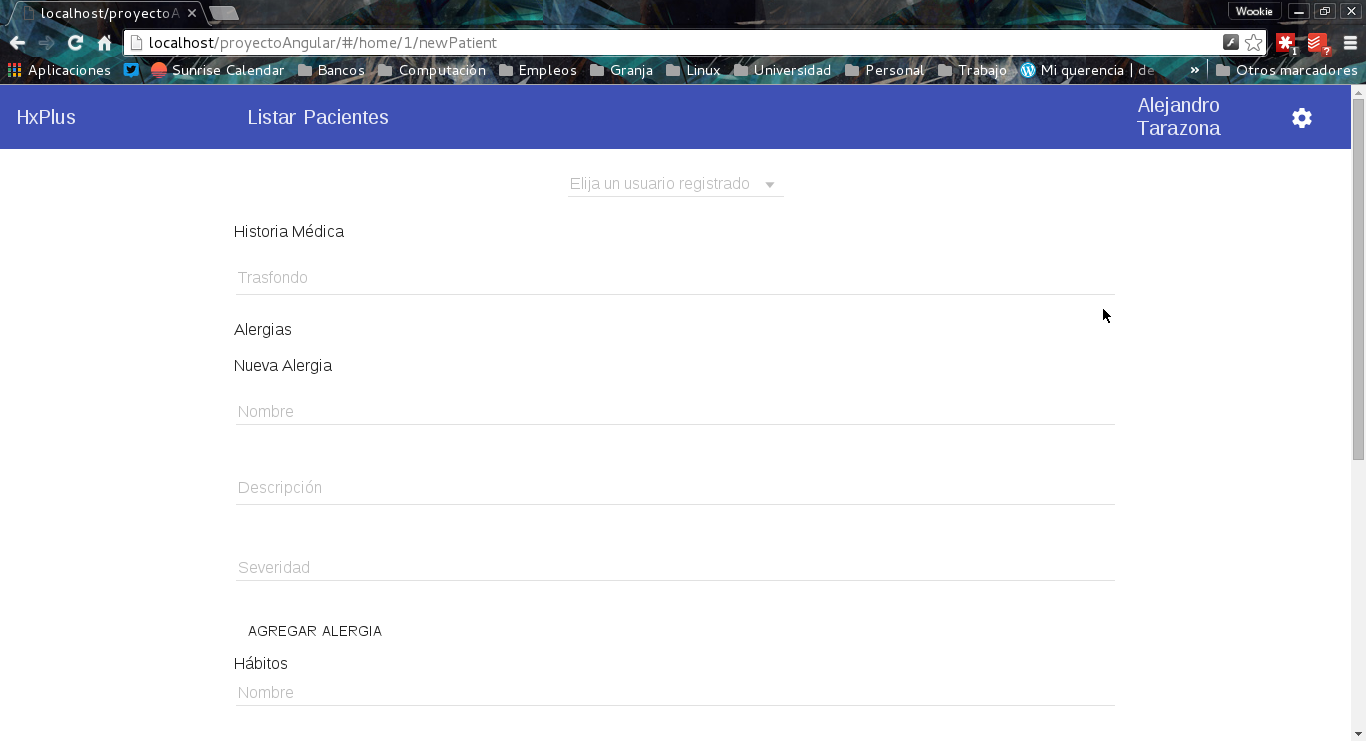
\includegraphics[width=.9\textwidth]{figures/p10}
        \end{center}
        \caption{Vista de creación de nueva historia médica para un paciente nuevo.}
        \label{creación}
    \end{figure}
    
    Debido a la complejidad de la implementación de los formularios dinámicos, se asignaron tres semanas para la implementación exitosa de esta vista. Las pruebas fueron realizadas basándose en:
    
    \begin{enumerate}
        \item Respuesta a agregación o eliminación de valores en los campos dinámicos.
        \item Carga y comunicación con el servidor.
        \item Revisión de la creación de la historia médica (por verificar luego de la implementación del punto \ref{historial-medico}).
    \end{enumerate}

    \subsection{Octavo Sprint: Vista de Agregar Consulta Médica}
    \label{crear-consulta}
    
    En esta vista se presentan los formularios respectivos para la creación de una nueva consulta médica separados por subvistas que van llenando cada una de los aspectos requeridos de las consultas médicas tal y como se enumeraron en \ref{consultas-datos} y subdivididos en:
    
    \begin{itemize}
        \item Resumen General:
            \begin{itemize}
                \item Análisis Subjetivo (\textit{Sujective})
                \item Análisis Objetivo (\textit{Objective})
                \item Plan de tratamiento
                \item Diagnóstico(s)\\
                En este caso se hizo uso de un formulario dinámico ya que pueden ser varios diagnósticos realizados en una misma consulta.
                \item Instrucción(es)\\
                También en este caso se realizó haciendo uso de los formularios dinámicos. Las instrucciones puede tener una o varias prescripciones médicas asociadas.
                \item Comentarios
            \end{itemize}
            
            \begin{figure}[htb!]
                \begin{center}
                    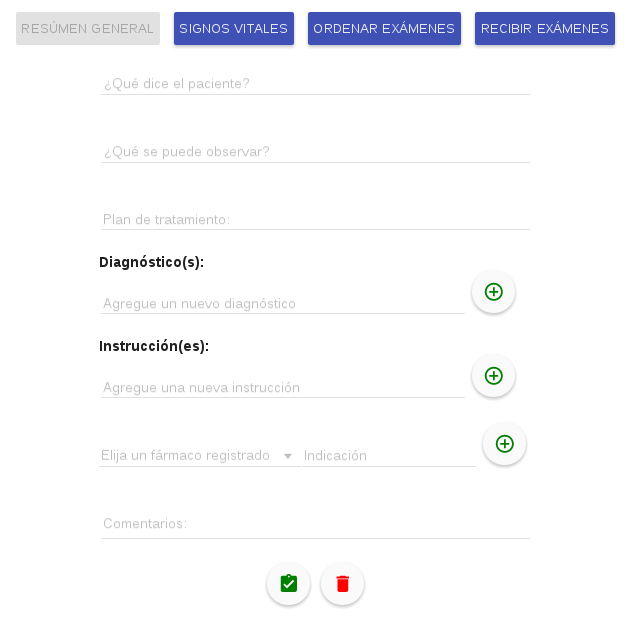
\includegraphics[width=.9\linewidth,keepaspectratio=true]{figures/consulta1}
                \end{center}
                \caption{Resumen General}
                \label{img-revisiongeneral}
            \end{figure}
                
        \item Signos Vitales:\\
        Para el caso en que aplique, se tiene esta sección de la consulta donde se registran los signos vitales tomados en la misma. Se tomó el nombre de ``Signos Vitales" por convención aunque refiere a datos fisiológicos en general: altura, peso, presión arterial y cualquier otro que el doctor considere pertinente. Se deja una acción especial para añadir al sistema nuevos parámetros; esto con la finalidad de permitir flexibilidad y mejorar la eficiencia de la carga de datos.
            \begin{itemize}
                \item Flexibilidad: En caso de precisar un nuevo parámetro fisiológico, por no estar previamente contemplado, el doctor puede agregarlo haciendo uso de la opción ``Otro".
                \item Carga de Datos: Dado que los parámetros requeridos pueden ser diferentes entre las disciplinas médicas, se estaría desperdiciando espacio en la base de datos si se tomara un sólo formulario con todos los parámetros registrados. Tomando en cuenta eso, se decidió que el doctor está en potestad de hacer la revisión del paciente y añadir los ``Signos Vitales" que considere pertinentes y que hayan sido medidos durante la consulta; así pues, un mismo doctor puede realizar dos consultas a un mismo paciente y en una registrar la ``temperatura corporal" (por ejemplo) y en otra consulta registrar la ``tensión arterial".
            \end{itemize}
            
            \begin{figure}[htb!]
                \begin{center}
                    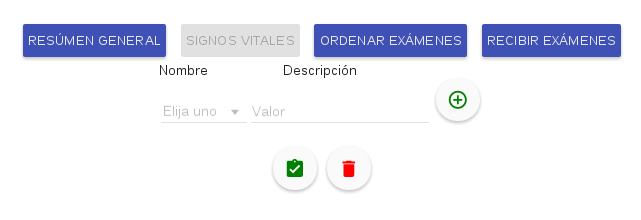
\includegraphics[width=.9\linewidth,keepaspectratio=true]{figures/consulta2}
                \end{center}
                \caption{Signos Vitales}
                \label{img-signovital}
            \end{figure}
        \item Solicitud de Examen Médico\\
        En este caso se utilizó un formulario dinámico para el registro de solicitud de exámenes médicos. En esta fase, el exámen sólo cuenta con un nombre, dado por el doctor tratante, y se registra la solicitud que puede ser recibida en una consulta futura en la sección ``Recibir Exámenes" descrita a continuación.
        
        \begin{figure}[htb!]
            \begin{center}
                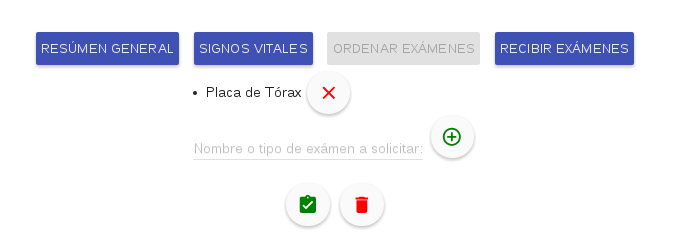
\includegraphics[width=.9\linewidth,keepaspectratio=true]{figures/consulta3}
            \end{center}
            \caption{Solicitud de Examen Médico}
            \label{img-solicitarexamen}
        \end{figure}
        
        \item Recepción de Examen Médico\\
        En esta fase el doctor puede indicar la recepción de un examen médico solicitado en una consulta previa, y sólo de los solicitados en consultas previas, junto con la carga de un archivo asociado al examen (en caso de poseer un archivo digital). La intención es mantener la información médica que llevó a diagnósticos de tal forma que se puedan realizar revisiones a la misma y estudios de evolución de pacientes. Ver figura \ref{img-recibirexamen}.
        
        \begin{figure}[htb!]
            \begin{center}
                
\includegraphics[width=.9\linewidth,keepaspectratio=true]{figures/consulta4}
            \end{center}
            \caption{Recepción de Examen Médico}
            \label{img-recibirexamen}
        \end{figure}
    \end{itemize}
    
    Para este Sprint, debido a la complejidad del formulario y la encapsulación de los datos requeridos, se asignó una duración de tres semanas en las cuales el equipo de desarrollo realizó la revisión de los tutoriales antes mencionados para lograr la correcta encapsulación de los datos.
    
    Para las pruebas de este Sprint se siguieron los siguientes parámetros:
    
    \begin{itemize}
        \item Respuestas y aceptación de UI.
        \item Encapsulación adecuada de los datos: Que los datos se preserven entre las distintas subvistas.
        \item Carga de datos en el sistema: Cantidad de datos y momento de transmisión.
        \item Formularios dinámicos y la respectiva carga de datos al formulario principal.
        \item Correctitud de los datos almacenados en el sistema.
    \end{itemize}
    
    Se dejó para el siguiente Sprint la revisión de la correcta carga de datos como la fecha para realizar la prueba conjunta con la revisión de la recuperación de datos de la vista \ref{historial-medico}.
    
    \subsection{Noveno Sprint: Vista de Historial de Consultas Médicas del Paciente}
    \label{historial-medico}
    
    En esta vista se presenta el historial completo de consultas médicas del paciente, ordenadas de manera cronológica y empezando por la última consulta. También se puede acceder a otros aspectos del historial médico, como por ejemplo hábitos, alergias, etc; tal y como se puede ver en la figura \ref{consultas}.
    
    \begin{figure}[htbp!]
        \begin{center}
            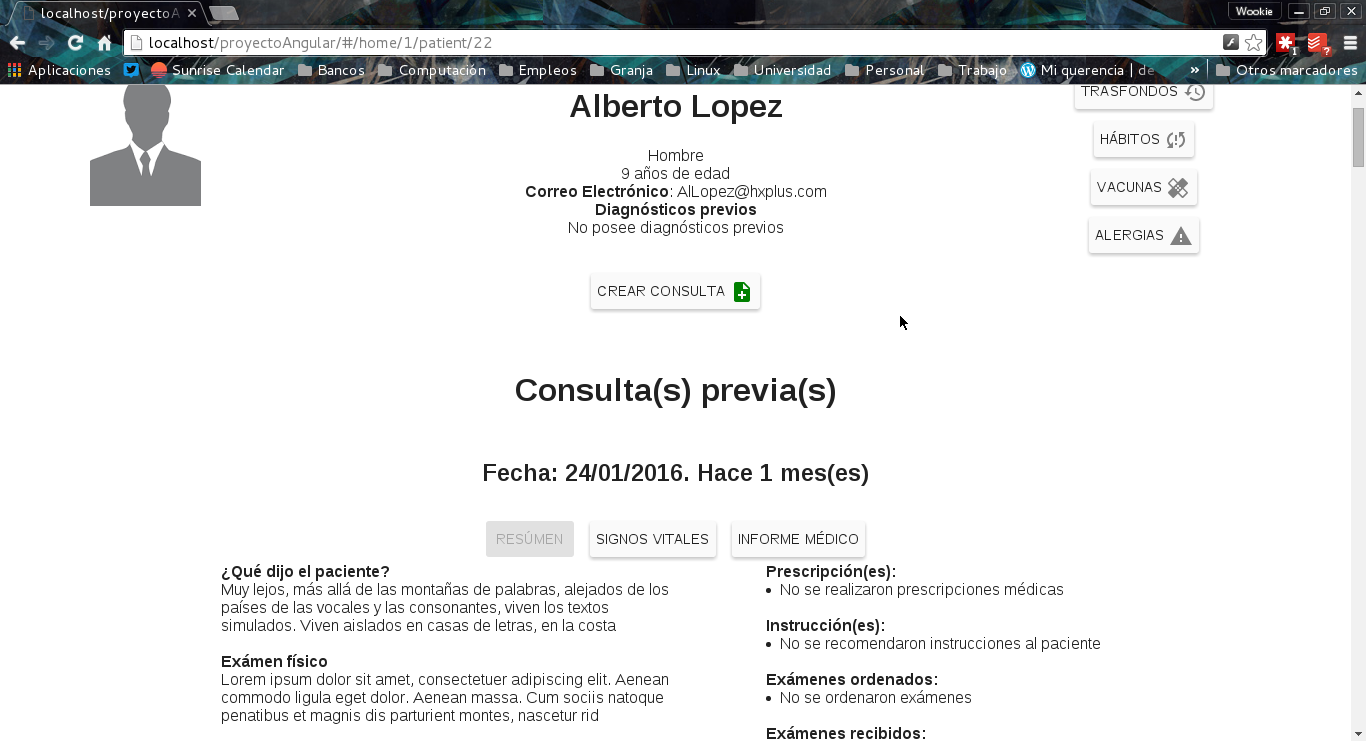
\includegraphics[    ]{figures/p11}
        \end{center}
        \caption{Vista de Historial de Consultas Médicas del Paciente}
        \label{consultas}
    \end{figure}
    
    La vista permite a su vez la integración con la vista de Revisión de Consulta Médica (ver \ref{revisar-consulta}) y Agregar Consulta (ver \ref{crear-consulta}).
    
    Las pruebas para esta vista fueron principalmente de aceptación de UI pero se tomó en cuenta la agregación de nuevas consultas a la lista una vez realizada la consulta y almacenada en el sistema. Además se revisó la integración con la vista de agregar consulta médica (ver \ref{crear-consulta}) y las acciones que ella realiza dentro del sistema.
    
    Para este Sprint se asignaron dos semanas pero debido a problemas de integración con las vistas mencionadas, fue requerido una semana adicional de revisión para el correcto funcionamiento de la vista.
    
    \subsection{Décimo Sprint: Vista de Revisión de Consulta Médica}
    \label{revisar-consulta}
    Esta vista está insertada en la vista anterior logrando que lo que se llama ``Historial Médico" de un paciente sea en sí la lista de todas las consultas médicas junto con los respectivos accesos a trasfondos, alergias, entre otros. La revisión de consulta médica se divide en dos fases:
    
    \begin{enumerate}
        \item Resumen\\
        Resumen general de la consulta, se muestra la \textit{Soap Note} de la consulta y los exámenes solicitados y recibidos (con su respectivo archivo, según coresponda).
        \item Signos Vitales\\
        En esta subvista se muestran los signos vitales recabados durante la consulta. Se muestra un mensaje adecuado en caso de no haberse recabado signos vitales durante dicha consulta. Se hace en un apartado para no saturar la vista principal de ``Resumen" con lo que es información muy específica y potencialmente puede ser excesiva para una vista ya cargada.
    \end{enumerate}
    
    Para este Sprint se asignaron dos semanas y las pruebas fueron realizadas tomando en cuenta:
    
    \begin{itemize}
        \item Integración con la vista \ref{historial-medico}.
        \item Actualización de los datos y revisión de los mismos al momento de agregar una nueva consulta (vista \ref{crear-consulta}).
        \item Aceptación de UI.
    \end{itemize}
    
    \begin{figure}[htb!]
        \begin{center}
            \begin{minipage}{0.45\textwidth}
                \begin{center}
                    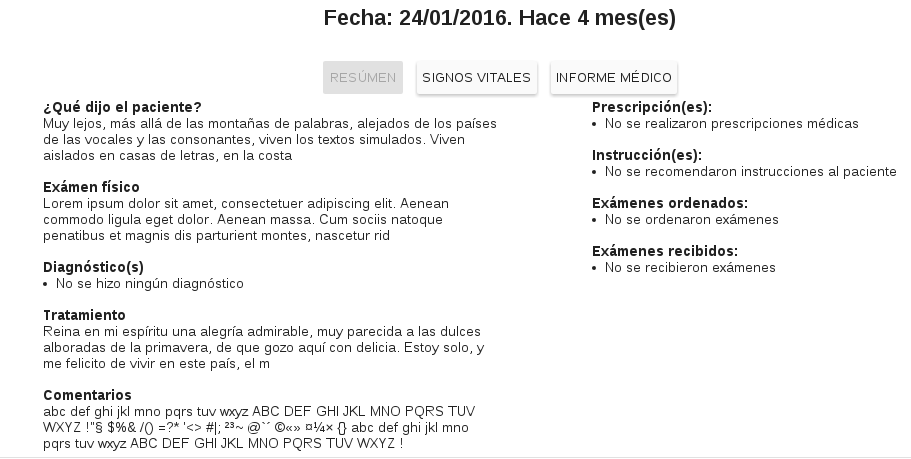
\includegraphics[width=\linewidth,keepaspectratio=true]{figures/consultarev-resumen}
                \end{center}
                \caption{Vista de Revisión de consulta. Resumen}
                \label{consultarev-resumen}
            \end{minipage}
            \hspace*{\fill}
            \begin{minipage}{0.45\textwidth}
                \begin{center}
                    
\includegraphics[width=\linewidth,keepaspectratio=true]{figures/consultarev-signosv}
                \end{center}
                \caption{Vista de Revisión de consulta. Signos Vitales}
                \label{consultarev-signosv}
            \end{minipage}
        \end{center}
    \end{figure}
    
    \subsection{Décimo Primer Sprint: Vista de Generación de Reportes Médicos}
    Esta vista se anexa a la ``Vista de Revisión de Consulta Méddica" como un apartado final. En ella el doctor puede generar un reporte con los datos de la consulta dada, seleccionando los que desea plasmar en dicho reporte, y descargar un archivo en formato PDF para ser entregado de manera digital o impreso directamente. También puede optar por generar un reposo médico, indicando la cantidad de días asignados a dicho reposo y descargando el archivo.
    
    En este punto el equipo de desarrollo precisó una semana de capacitación por la utilización de iText (ver punto \ref{tecno-itext}) herramienta que fue la elegida para la generación de archivos PDF y que hasta el momento no había sido utilizada en el desarrollo.
    
    Tomando en cuenta la semana de capacitación, este Sprint contó con una duración de dos semanas y las pruebas fueron basadas en:
    
    \begin{itemize}
        \item Aceptación de UI.
        \item Correctitud de la información en el informe médico generado.
        \item Correctitud de la información en los reposos médicos.
        \item Aceptación del formato visual de ambas clases de archivos.
    \end{itemize}
    %  Informe
    \begin{figure}[htb!]
        \begin{minipage}{0.45\textwidth}
            \begin{center}
                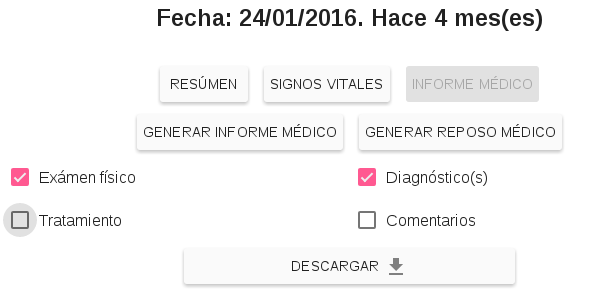
\includegraphics[width=\linewidth,keepaspectratio=true]{figures/reportes-informenav}
            \end{center}
            \caption{Vista de Generación de Reportes Médicos. Informe}
            \label{reportes-informenav}
        \end{minipage}
        \hspace*{\fill}
        \begin{minipage}{0.45\textwidth}
            \begin{center}
                
\includegraphics[width=\linewidth,keepaspectratio=true]{figures/reportes-informepdf}
            \end{center}
            \caption{Archivo de informe médico generado por el sistema}
            \label{reportes-informepdf}
        \end{minipage}
    \end{figure}
    
    %  Reposo
    \begin{figure}[htb!]
        \begin{minipage}{0.45\textwidth}
            \begin{center}
                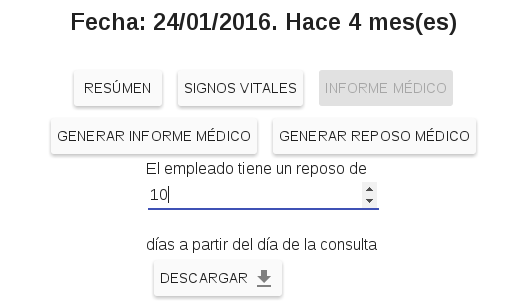
\includegraphics[width=\linewidth,keepaspectratio=true]{figures/reportes-reposonav}
            \end{center}
            \caption{Vista de Generación de Reportes Médicos. Reposo}
            \label{reportes-reposonav}
        \end{minipage}
        \hspace*{\fill}
        \begin{minipage}{0.45\textwidth}
            \begin{center}
                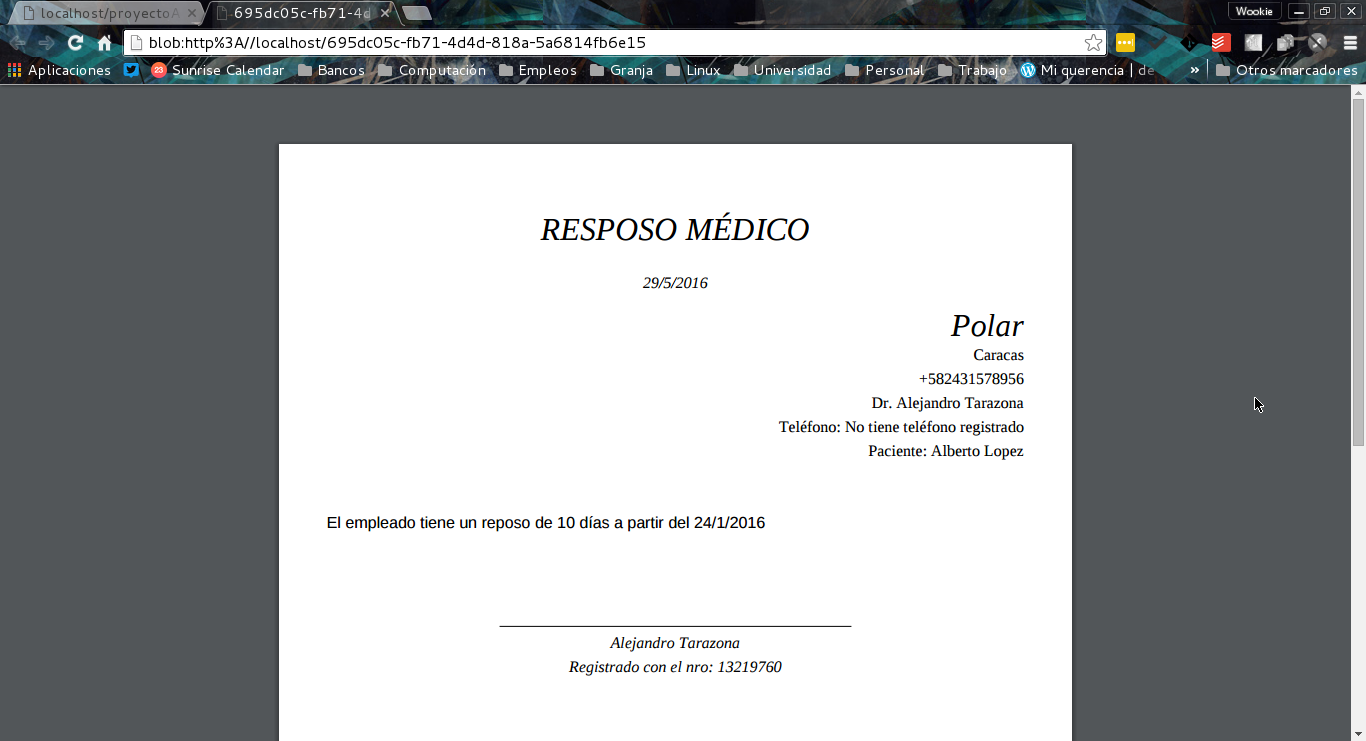
\includegraphics[width=\linewidth,keepaspectratio=true]{figures/reportes-reposopdf}
            \end{center}
            \caption{Archivo de reposo médico generado por el sistema}
            \label{reportes-reposopdf}
        \end{minipage}
    \end{figure}
    
    
\section{Fase de Cierre}

\subsection{Dificultades generales encontradas}

    Las dificultades encontradas durante el desarrollo del proyecto fueron:
    
    \begin{itemize}
        \item \textbf{Restricción en el uso de herramientas:} el \textit{Product Owner} solicitó explícitamente el uso de Java, SPRING, Hbernate, JavaScript, MySQL, AngularJS y JSON, tal y como fue descrito, para el desarrollo. Lo cual, si bien facilitó la creación y desarrollo del proyecto, dejó imposibilitada la posibilidad de, con tecnologías actuales, dar soporte a una base de datos orientada a eventos, tal como se pretendía hacer al principio.
        
        \item \textbf{Falta de informción de parte de Inpsasel:} originalmente se buscaba generar informes médicos especializados para el reporte de enfermedades ocupacionales al Inpsasel, órgano encargado de la gestión de enfermedades ocupacionales en el émbito nacional. Sin embargo, la falta de información, formatos y, más adelante, el lanzamiento de su portal (de Inpsasel) con automatización de dicha gestión, dejó a HxPlus Ocupacional sin la necesidad de realizar dichos informes.
    \end{itemize}
    
    \subsection{Resultados Generales}
    
    El proyecto de pasantía se completó satisfactoriamente. A pesar de no poseer la funcioncionalidad de generación de informes de Inpsasel, la empresa de consideró satisfecha con los módulos implementados. La línea de tiempo de consultas se muestra adecuadamente y en orden cronológico, los diagnósticos y planes son almacenados y mostrados a gusto de la empresa y de conformidad con los lineamientos.
    
    Queda de parte de la empresa gestionar el desarrollo de futuros módulos o funcionalidades para la aplicación.
        